The two major contributions of this work are summarized as follows:

\begin{itemize}
    \item Implementation of a flexible deep reinforcement learning framework that can be extended to learn new 
    reinforcement learning problems in the RoboCup Soccer Simulation 3D environment. The source code was made 
    available online and is referenced in Section \ref{sec:envandimpl}.
    \item Providing the task modelling and setup of 3 simulated humanoid tasks.
    With these specifications it is possible to reproduce this work's results and learn similar tasks with minor
    modifications. Specifically, this entitles the framing
    of the problems as a RL task and the learning algorithms to successfully learn these tasks.
\end{itemize}

\section{Environment and Implementation}
\label{sec:envandimpl}

In the early stages of the project, we implemented a working version of DDPG that could successfully learn some classical continuous control
problems from OpenAI Gym.
For example, we mastered the inverted pendulum swingup toy problem that consists of a pendulum that starts in a random position, 
and the goal is to swing it up so it stays upright.
This process of implementing the algorithms from scratch was very time consuming because Deep RL algorithms are hard to validate \cite{VerificationRL}.

However, since we would experiment with multiple algorithms, we decided to use readily available RL algorithms
implementations. The implementation of PPO, TRPO and DDPG algorithms are from the OpenAI Baselines repository \cite{OpenAIBaselines}. 
OpenAI Baselines is a GitHub repository with a set of high-quality implementations of reinforcement learning algorithms.
Not implementing all the DRL algorithms from scratch made it much easier to experiment with new algorithms. 

The project is composed of two main modules (each of them running as a separate process):
\begin{itemize}
    \item \textbf{Learning Client:} Process that runs the reinforcement learning algorithms and makes remote procedure calls (RPCs)
    to the server exchanging state/action information of the soccer agent. This module was implemented in Python 3.5 and TensorFlow using the
    OpenAI Baselines \cite{OpenAIBaselines} implementations.
    \item \textbf{Soccer Agent:} Process that interacts with SimSpark and that interacts with the learning client.
    This module was implemented in C++ and uses the ITAndroids Soccer Simulation 3D code base.
\end{itemize}

The API between the the server and the client uses Protocol Buffers and its communication is done between RPCs 
that exchange state-action information on every update loop.

A general diagram is depicted in Figure \ref{fig:architecture}. Notice that the Simulation Server is SimSpark
and we have no control over its update loop.

\begin{figure}[H]
    \centering
    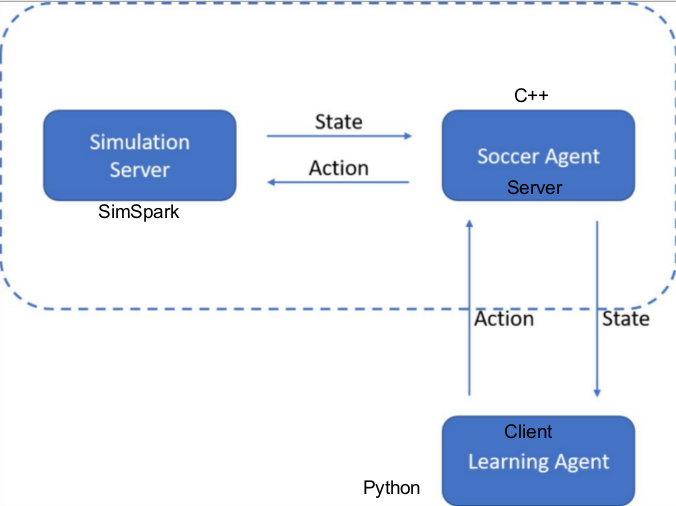
\includegraphics[width=0.95\textwidth]{Chapter5/architecture.png}
    \caption{Learning Architecture diagram.}
    \label{fig:architecture}
\end{figure}

This uncoupled design between the server and the client enabled us to easily change the learning algorithms 
in the client while not influencing the server and allowed us to switch tasks transparently in regards to the client.
This project lays the groundwork for the ITAndroids 3D Soccer Simulation team to use DRL for learning other
behaviors. Also, other teams from the 3D Soccer Simulation league could benefit from using the code to learn additional
 behaviors since the implementation is easily extensible.
The source code for the client is available at:

\url{https://github.com/alexandremuzio/ddpg-humanoid}.


\section{Task Modelling}
\label{sec:tasks}

The main task we are trying to solve is of learning a soccer dribbling behavior.
We also learn $2$ much simpler problems that we call warm-up tasks. 
Learning these additional task was very helpful to get a better understanding
of the simulation environment and of how the reward shaping should be.

In this section we fully describe the tasks: the state space, action space and the reward signal of each task.
Let ($x$, $y$, $z$ and $\theta$) be the absolute pose variables, as shown in Figure \ref{fig:robotpos}. 
These variables constitute part of the agent's space and retrieved from the server using the Wizard (ground truth).
The speed for each of these variables is calculated by the ratio of the difference between $2$ consecutive measurements by the timestep duration.

\begin{figure}[H]
    \centering
    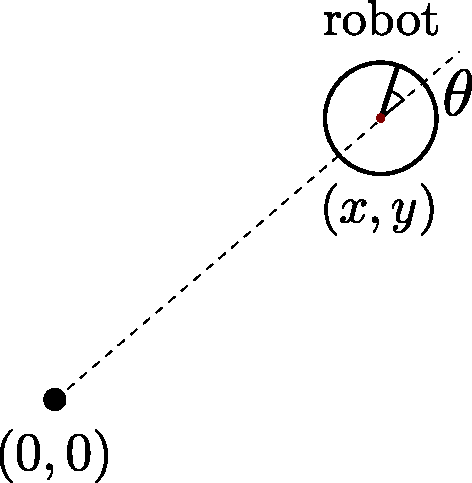
\includegraphics[width=0.4\textwidth]{Chapter6/robot_pos.pdf}
    \caption{Robot pose representation.}
    \label{fig:robotpos}
\end{figure}

For example, to calculate the frontal speed, $v_x$ from $x_t$ and $x_{t-1}$, $x$ coordinates of the robot at timestep $t$ and $t-1$ respectively,
and the duration of the timestep, $\Delta t$, we use 

\begin{align*}
    v_x = \dfrac{x_t - x_{t-1}}{\Delta t}
\end{align*}

We calculate $v_y$ and $v_{\theta}$ analogously.
However, since calculating speed by deriving position is very noisy, we use a low-pass filter to smooth out the signal. 

\section{Humanoid Speed Walker Task (Warm-Up)}

This task is basically for the simulated robot agent to learn how to to walk forward with constant reference speed that we denote by $v_{ref}$.
It is a simple problem to get a better intuition of how the environment works.

\textbf{State space:} the 1D observations consists only on the frontal robot velocity $v_x$.

\textbf{Action space:} the 1D action space consists of the commanded frontal speed $u_x$ to be executed by the
walk engine.

\textbf{Reward signal:} The reward is given by:
\begin{align*}
    r(s,a) = \mathbb{I}^{\text{close to ref}} - 100 \mathbb{I}^{\text{robot fell}}
\end{align*}
where $\mathbb{I}^{\text{close to ref}}$ equals $1$ if $\lvert v_{ref} - v_x \rvert < \epsilon$ and $0$ otherwise; and 
$\mathbb{I}^{\text{robot fell}}$ equals $1$ if the robots has fallen and $0$ otherwise.
We define that the robot has fallen if $z_{CoM} < 0.2$.
The episode terminates after $T$ = 2000 steps or if the robot falls.

\section{Humanoid Racing Task (Warm-Up)}

This task describes a race track of $18$x$4$m  in which the robot must 
reach the finish line while remaining between the two lanes.

Figure \ref{fig:racer_domain} illustrates the task as shown in \textit{RoboViz}. 
The simulated Nao robot starts the race on the center of the green line and tries to reach the red
finish lines without crossing the black border lines.

\begin{figure}[ht]
    \centering
    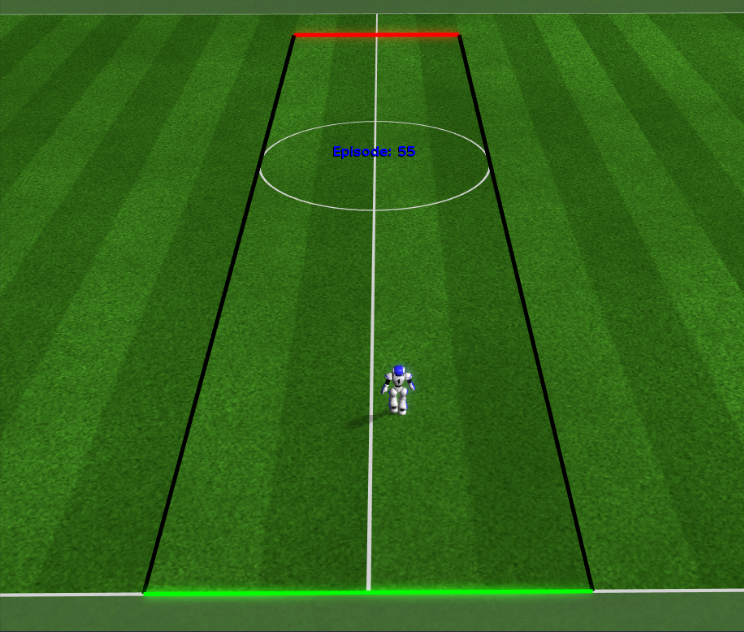
\includegraphics[width=1.0\textwidth]{Chapter6/racer_domain.png}
    \caption{Humanoid Racing Domain.}
    \label{fig:racer_domain}
\end{figure}

\textbf{State space:} the observations consists of the $x$, $y$, $z$ coordinates of the torso, the yaw
angle of the torso, the forward speed $v_x$, sideways speed $v_y$ and rotational speed $v_{\theta}$.

\textbf{Action space:} the 3D action space consists of $u_x$, $u_y$ and $u_{\theta}$, speed control signal
in forward, sideways and rotational directions, respectively.

\textbf{Reward signal:} the reward is defined by:
\begin{equation*}
    \begin{aligned}
    r(s,a) = v_x - 0.005 (v_{\theta}^2 + v_y^2) - 0.05 (u_{x}^2 + u_{y}^2 + u_{\theta}^2) -  0.05 y^2 \\
        + 50 \mathbb{I}^{\text{finish line}} - 10\mathbb{I}^{\text{leave track}} - 10\mathbb{I}^{\text{robot fell}}
\end{aligned}
\end{equation*}
where $\mathbb{I}^{\text{finish line}} = 1$ if the robot arrives the finish line and $0$ otherwise; and 
$\mathbb{I}^{\text{leave track}} = 1$ if the robot leaves the track and $0$ otherwise.

The term $v_x$ rewards the robot for moving in the direction of the race track and the terms $-0.05 (v_{\theta}^2 + v_y^2)$ 
and $-0.05 y^2$  penalize deviation from the forward direction. This was inspired by \cite{BenchmarkingDRL}.

The episode duration is $2000$ steps and the episode terminates if the robot falls ($z_{CoM} < 0.2$)
or if the robot leaves the race track.

%%%%%%%%%%%%%%
\section{Humanoid Soccer Dribbling Task}

The task describes a $4$x$3$m rectangle in which there is one learning agent and one opponent agent fighting to take control of the ball.
This task's goal is for the robot to take control of the ball and dribble it past the opponent to the right end side of the rectangle.
We assume that the better the agent performs on this task, the better it performs at the task of dribbling on its own.
We shall refer to the robot that is not being trained as the opponent.

Figure \ref{fig:soccerdomain} depicts this task as seen by the monitor. 
The yellow lines denote the task bounds, the blue agent is the agent being trained and the red agent is the
opponent player. Also, note that the blue/red lines in front of the agent denote the robot's torso orientation and
were only drawn for visualization purposes.

\begin{figure}[ht]
    \centering
    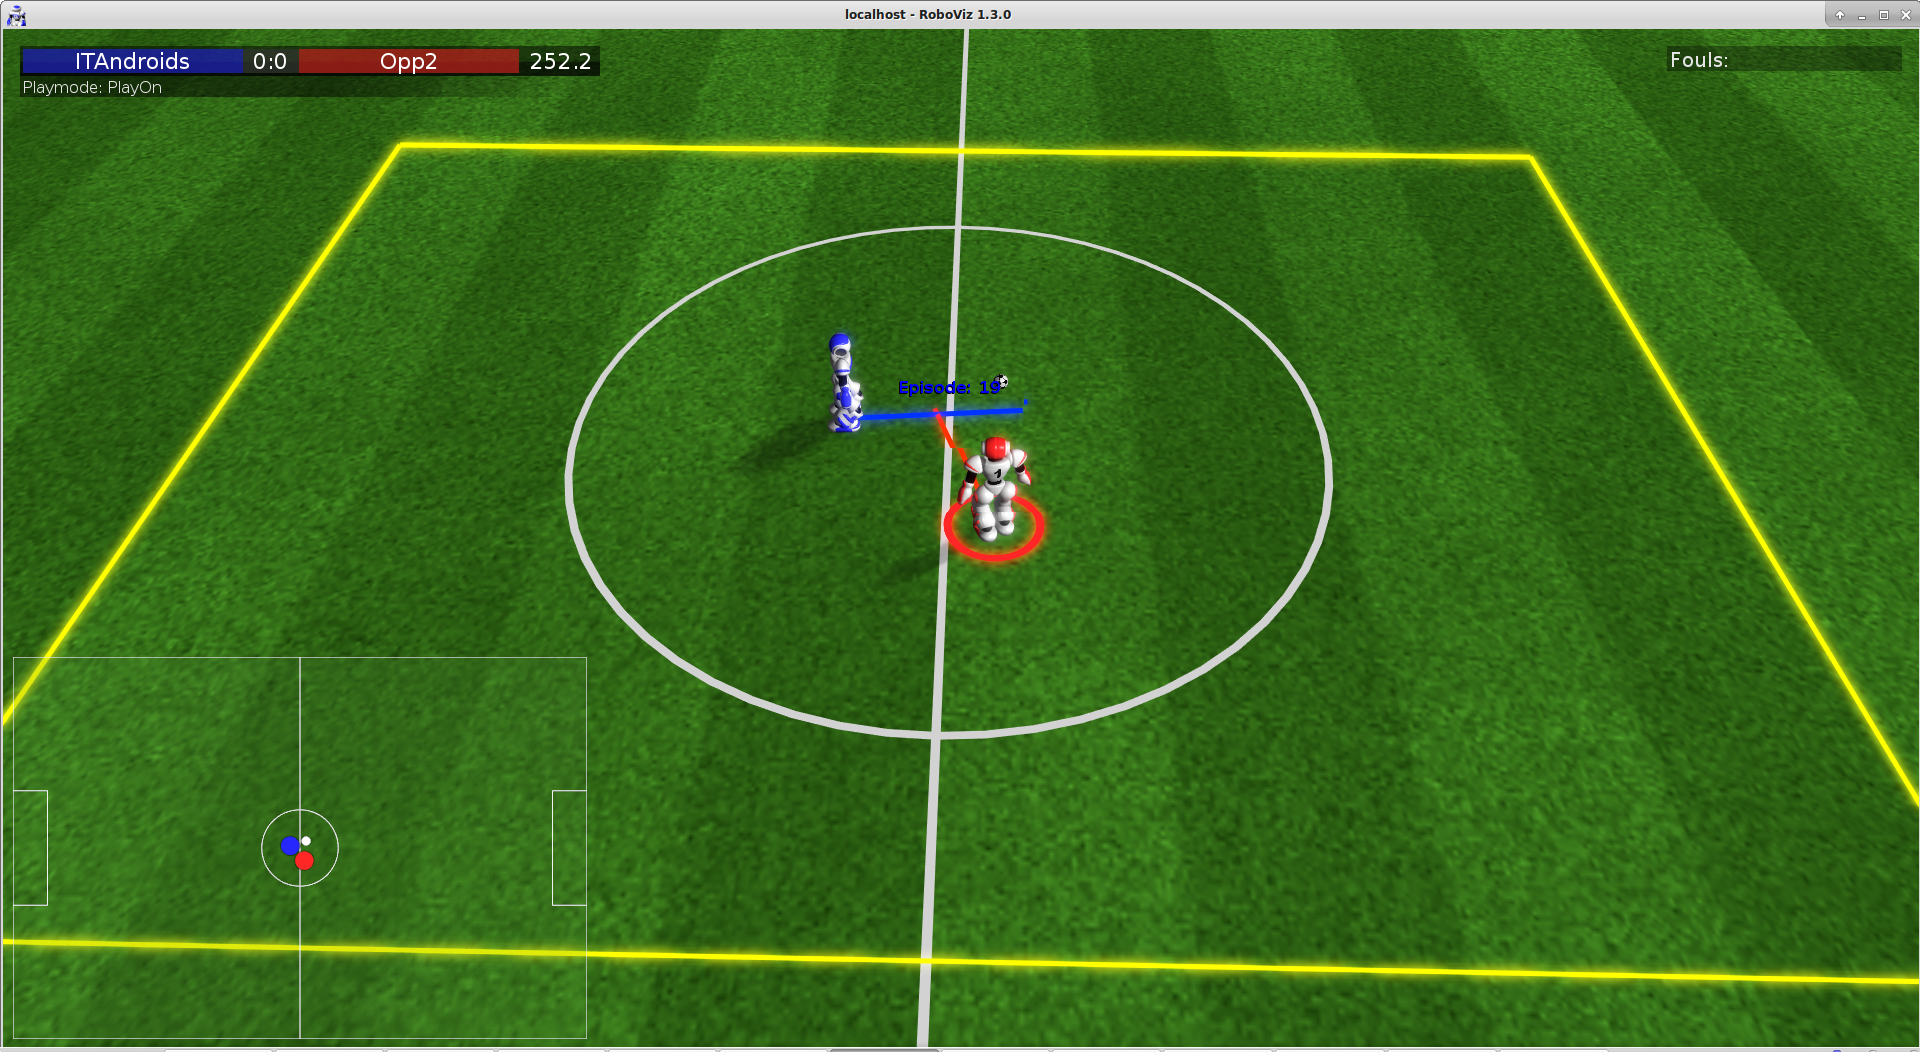
\includegraphics[width=1.0\textwidth]{Chapter6/soccer_domain.png}
    \caption{Humanoid Soccer Dribbling Domain.}
    \label{fig:soccerdomain}
\end{figure}

This is the most challenging of the tasks presented and is where we mainly focus our effort.

\textbf{State space:} the observations consists of the $x$, $y$, $z$ coordinates of the torso, the yaw
angle of the torso, the forward speed $v_x$, sideways speed $v_y$ and rotational speed $v_{\theta}$.
Also, the relative pose of the ball to the agent, the relative pose of the opponent to the agent and 
the relative pose of the ball to the opponent is used. We also found that using the ball-agent, ball-opponent and
agent-opponent improved learning performance.

\textbf{Action space:} the 3D action space consists of $u_x$, $u_y$ and $u_{\theta}$, speed control signal
in forward, sideways and rotational directions, respectively.

\textbf{Reward signal:} the reward is defined by:
\begin{equation*}
    \begin{split}
r(s,a) = (d^{t-1}_{\text{ball-agent}} - d^{t}_{\text{ball-agent}}) + 0.05 e^{(-d^{t}_{\text{ball-agent}})} \\
- (d^{t-1}_{\text{opp-agent}} - d^{t}_{\text{opp-agent}}) + 5 \Delta x_{\text{ball}} \\
+ 10 \mathbb{I}^{\text{agent completed dribble}} -10 \mathbb{I}^{\text{opp completed dribble}}  - 1 \mathbb{I}^{\text{agent fell}} 
\end{split}
\end{equation*}
where $\mathbb{I}^{\text{agent completed dribble}} = 1$ if the agent successfully completed the dribble and $0$ otherwise; and 
$\mathbb{I}^{\text{opp completed dribble}} = 1$ if the opponent successfully completed the dribble and $0$ otherwise.
The term $\Delta x_{\text{ball}}$ is the difference in the $x$ axis for the ball in one timestep and rewards the agent
for pushing the ball forward -- in the direction of a successful dribble.
The term $e^{(-d^{t}_{\text{ball-agent}})}$ rewards the robot for the closer it is to the ball.
Finally, the term $ (d^{t-1}_{\text{ball-agent}} - d^{t}_{\text{ball-agent}})$ rewards the agents for moving in the direction
of the ball (analogously for the opponent term).

Unfortunately, some reward engineering was needed, since dribbling inherently has very sparse rewards.
We based the reward signal on some ideas from \citen{2017-TOG-deepLoco,BenchmarkingDRL}.

The episode duration is $5000$ steps and the episode terminates if the following events take place: 

\begin{itemize}
    \item Agent falls: $z_{CoM} < 0.2$.
    \item Agent leaves task areas.
\end{itemize}

Notice that if the opponent leaves the field, we simply respawn it back to the field.

\subsection{Curriculum}

To successfully learn this task, we used a learning curriculum \cite{BengioCurrLearning}.
The curriculum aids exploration in the environment since it increases the probability of success of
the agents by yielding positive reward from random actions \cite{OpenAISelfPlay}.

The curriculum we used for this task is composed of two parts:

\begin{itemize}
    \item Agent-ball distance in the start of the episode. During learning, at each new episode, the agent spawns at a random position relative 
    to the ball. However the curriculum we use specifies that the maximum distance the agent can start from the ball increases
    over the duration of the training.
    The idea is that we want to increase the probability that the agent dribbles the ball forward, yielding a high reward.
    \item Opponent skill. We use two opponents with different skill levels. During the start of the training,
    we start the opponent off with a lower skill level and change it to the one with the higher skill level.
    Basically, the lower level agent does not move and the skilled agent is the ITAndroids implemented
    dribble agent that uses classical control theory.
\end{itemize}

Using a curriculum was fundamental to successfully learn this task. If we did not control the opponent
skill, the agent would not randomly receive high rewards for completing the dribble only with a 
random policy.
